\subsection{Display driver}

The display driver consists of a hardware and a software part. Since the display runs best at 3.3V, we decided to make a small circuit to facilitate this, even though it says in the data sheet of the display\cite[p. 17]{philips:pcd8544} that it can run on 5V.

\subsubsection{PCD8544 - Hardware}

Interfacing the display, we are using a hex buffer that we supply with 3.3V. This enables us to run the output from the microprocessor to the buffer at 5V, and the buffer shifts the level down to 3.3V\cite[p. 1]{STMicroelectronics:HCF4050B}.

To make the 3.3V, we are using an LM317L that can take the 5V supplied by the STK500 kit and convert it to 3.3V. This small circuit can be seen in figure \ref{fig:pcd8544_circuit}.

\begin{figure}
	\centering
	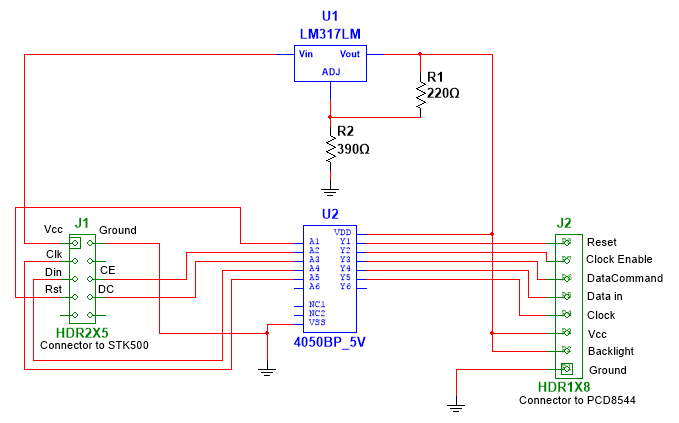
\includegraphics[width=.75\textwidth]{implementation/pcd8544_circuit}
	\caption{3.3V circuit}
	\label{fig:pcd8544_circuit}
\end{figure}

The circuit is quite simple and consist of the LM317L, the HCF4050B hex buffer and two resistors for the LM317L. All the hex buffer does is change the level of the inputs from the ATmega32 and outputs those to the screen.

\subsubsection{PCD8544 - Software}

For the software part of the display, there are a couple of things that we need to focus on. Firstly, there is a clear and easy way to reset the panel to a known state. After the reset we need to setup the display. 
This consists of setting the bias and the voltage to the LCD driver.

\subsubsection{Setup}

First, we need to issue a reset to the screen.

\begin{figure}
	\centering
	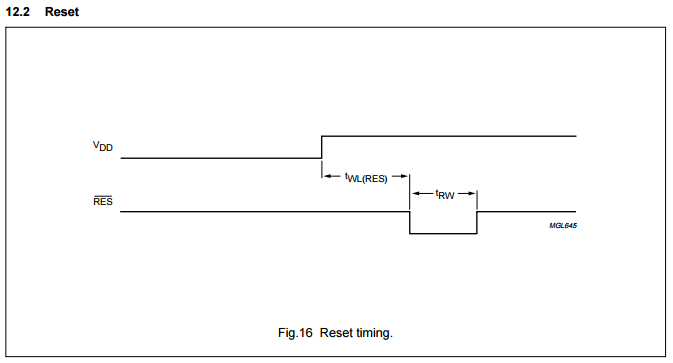
\includegraphics[width=.6\textwidth, trim={1cm 25mm 1cm 25mm}, clip]{implementation/pcd8544_resetTiming}
	\caption{Reset state for the PCD8544\cite[21]{philips:pcd8544}}
	\label{fig:pcd8544_resetTiming}
\end{figure}

As seen in Figure~\ref{fig:pcd8544_resetTiming}, we need to pull the \texttt{Reset} pin low to reset the panel. The reset has to occur within 0-30ms of the VCC going high\cite[20]{philips:pcd8544}. The reset line needs to be low for a minimum of 100ns\cite[20]{philips:pcd8544}.

The state of the display after a reset can be seen in figure~\ref{fig:pcd8544_reset}.

\begin{figure}
	\centering
	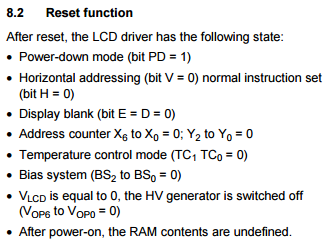
\includegraphics[width=.4\textwidth]{implementation/pcd8544_reset}
	\caption{Reset state for the PCD8544\cite[15]{philips:pcd8544}}
	\label{fig:pcd8544_reset}
\end{figure}

In Figure~\ref{fig:pcd8544_reset}, we can see that we need to tweak a few things to setup the display. We need to set the power mode to active and we need to change to the extended instruction set, so that we can set the operation voltage.

After this we need to change back to the basic instruction set and set the display mode. In our case, we want normal.

Since the RAM contents are undefined, we should also set these to a known state. After we have done this, we should be ready to use the panel.

\subsubsection{Transferring data/commands}

Since we are using the SPI driver for communication, all we need to concern ourselves with is the transferring data and command settings, the \texttt{SCE} (Serial Clock Enable) pin and the \texttt{D/C} (Data/Command) pin.

\begin{figure}
	\centering
	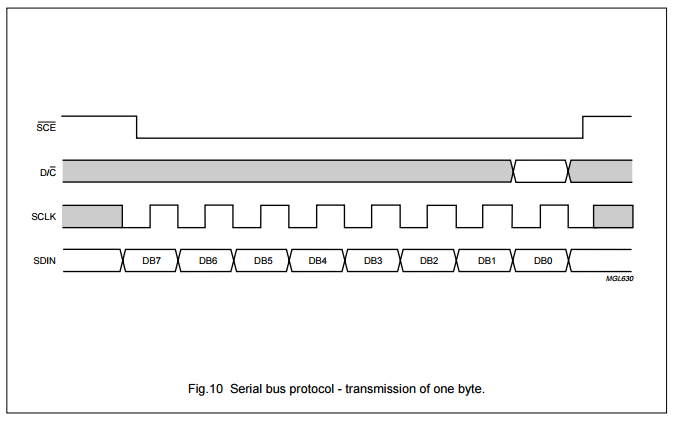
\includegraphics[width=.6\textwidth]{implementation/pcd8544_transmission}
	\caption{Transmission of one byte for the PCD8544\cite[p. 12]{philips:pcd8544}}
	\label{fig:pcd8544_transmission}
\end{figure}

In Figure~\ref{fig:pcd8544_transmission}, we see the transmission of one byte.
From this we can see that \texttt{SCE} has to be held LOW for the duration of the transmission, and that the \texttt{D/C} has to be set when the last bit is read.

If we do not pull the \texttt{SCE} HIGH again after we are done, the display will look for another byte transmission. We can use this fact to write the entire screen at once. This could e.g. be an array representation of the display, that we have in RAM.

\subsubsection{Commands}

The screen has a lot of instructions for setup.

\begin{figure}
	\centering
	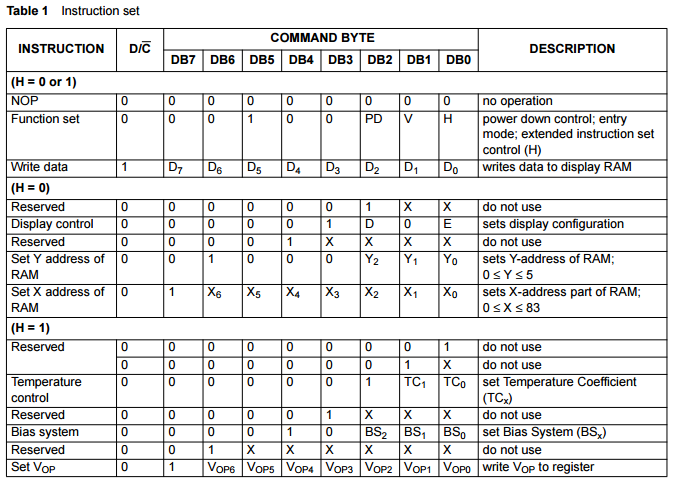
\includegraphics[width=.5\textwidth]{implementation/pcd8544_instructions}
	\caption{Transmission of one byte for the PCD8544\cite[p. 12]{philips:pcd8544}}
	\label{fig:pcd8544_Instructions}
\end{figure}

As seen in Figure~\ref{fig:pcd8544_Instructions}, the display has two instruction sets: one called basic and one called extended. To be able to use all of these commands, you can switch between the two with the function command.

The driver implements all the instructions for the user, but it is up to the user to know whether the display is in extended or basic mode. This was done to allow for sending more than one instruction and not having to change instruction set all the time.
